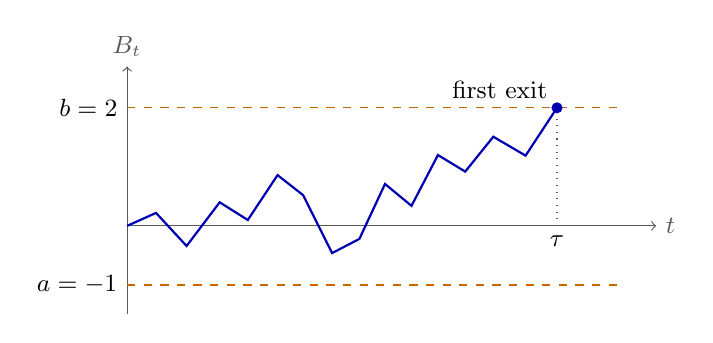
\begin{tikzpicture}[x=1.05cm,y=0.75cm]
\draw[->,black!65] (0,0)--(6.4,0) node[right,font=\small] {$t$};
\draw[->,black!65] (0,-1.5)--(0,2.7) node[above,font=\small] {$B_t$};
\draw[dashed,orange!80!black] (0,2)--(6,2);
\draw[dashed,orange!80!black] (0,-1)--(6,-1);
\node[left,font=\small] at (0,2) {$b=2$};
\node[left,font=\small] at (0,-1) {$a=-1$};
\draw[blue!70!black,thick] (0,0)--(0.35,0.22)--(0.72,-0.34)--(1.12,0.4)--(1.46,0.1)--(1.82,0.86)--(2.13,0.52)--(2.48,-0.46)--(2.81,-0.22)--(3.12,0.71)--(3.44,0.34)--(3.76,1.2)--(4.09,0.92)--(4.43,1.51)--(4.82,1.19)--(5.2,2);
\draw[dotted,black!65] (5.2,0)--(5.2,2);
\fill[blue!70!black] (5.2,2) circle[radius=2pt];
\node[below,font=\small] at (5.2,0) {$\tau$};
\node[above left,font=\small] at (5.2,2) {first exit};
\end{tikzpicture}
